\usetikzlibrary{trees, shadows, positioning, shapes.geometric, arrows.meta}

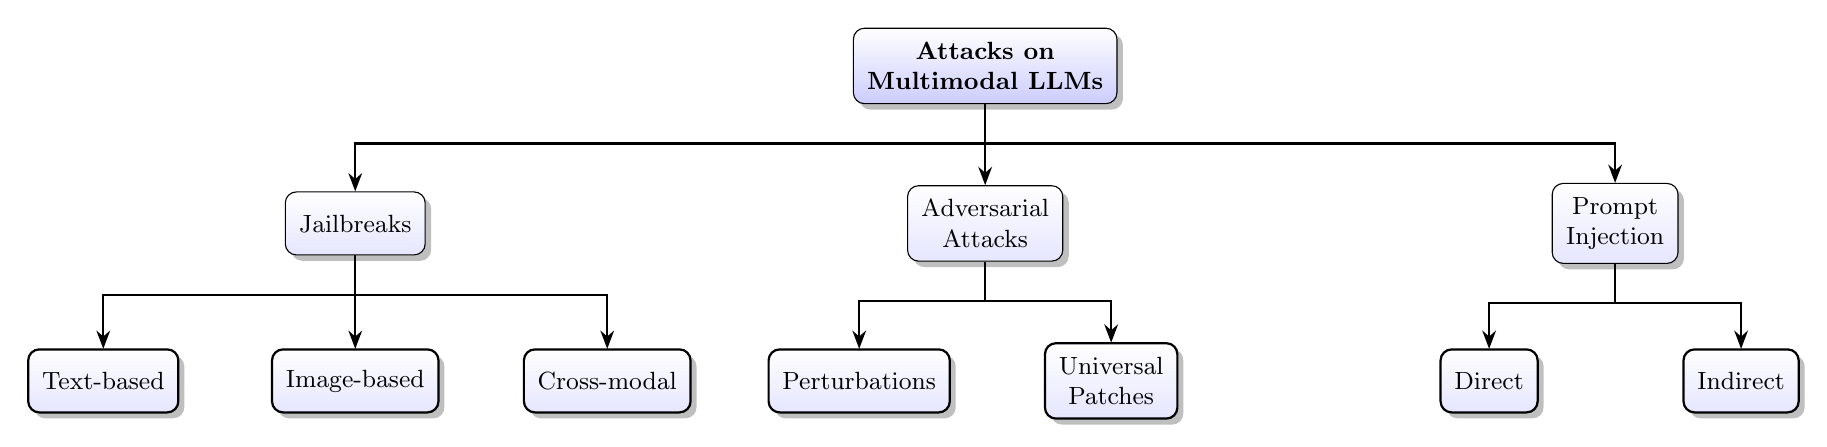
\begin{tikzpicture}[
    level 1/.style={sibling distance=8cm, level distance=2cm},
    level 2/.style={sibling distance=3.2cm, level distance=2cm},
    every node/.style={
        draw,
        rectangle,
        rounded corners,
        align=center,
        top color=white,
        bottom color=blue!10,
        drop shadow,
        font=\small,
        minimum height=0.8cm,
        inner sep=5pt
    },
    edge from parent/.style={
        draw,
        ->,
        thick,
        >=Stealth
    },
    edge from parent path={
        (\tikzparentnode.south) -- ++(0,-0.5cm) -| (\tikzchildnode.north)
    }
]

\node[bottom color=blue!20, font=\small\bfseries] {Attacks on\\Multimodal LLMs}
    child {node {Jailbreaks}
        child {node {Text-based}}
        child {node {Image-based}}
        child {node {Cross-modal}}
    }
    child {node {Adversarial\\Attacks}
        child {node {Perturbations}}
        child {node {Universal\\Patches}}
    }
    child {node {Prompt\\Injection}
        child {node {Direct}}
        child {node {Indirect}}
    };

\end{tikzpicture}
